%
\documentclass{sigchi}

% Use this command to override the default ACM copyright statement
% (e.g. for preprints).  Consult the conference website for the
% camera-ready copyright statement.

%% HOW TO OVERRIDE THE DEFAULT COPYRIGHT STRIP --
%% Please note you need to make sure the copy for your specific
%% license is used here!
% \toappear{
% Permission to make digital or hard copies of all or part of this work
% for personal or classroom use is granted without fee provided that
% copies are not made or distributed for profit or commercial advantage
% and that copies bear this notice and the full citation on the first
% page. Copyrights for components of this work owned by others than ACM
% must be honored. Abstracting with credit is permitted. To copy
% otherwise, or republish, to post on servers or to redistribute to
% lists, requires prior specific permission and/or a fee. Request
% permissions from \href{mailto:Permissions@acm.org}{Permissions@acm.org}. \\
% \emph{CHI '16},  May 07--12, 2016, San Jose, CA, USA \\
% ACM xxx-x-xxxx-xxxx-x/xx/xx\ldots \$15.00 \\
% DOI: \url{http://dx.doi.org/xx.xxxx/xxxxxxx.xxxxxxx}
% }

% Arabic page numbers for submission.  Remove this line to eliminate
% page numbers for the camera ready copy
% \pagenumbering{arabic}

% Load basic packages
\usepackage{balance}       % to better equalize the last page
\usepackage{graphics}      % for EPS, load graphicx instead 
\usepackage[T1]{fontenc}   % for umlauts and other diaeresis
\usepackage{txfonts}
\usepackage{mathptmx}
\usepackage[pdflang={en-US},pdftex]{hyperref}
\usepackage{color}
\usepackage{booktabs}
\usepackage{textcomp}


% Some optional stuff you might like/need.
\usepackage{microtype}        % Improved Tracking and Kerning
% \usepackage[all]{hypcap}    % Fixes bug in hyperref caption linking
\usepackage{ccicons}          % Cite your images correctly!
% \usepackage[utf8]{inputenc} % for a UTF8 editor only

% If you want to use todo notes, marginpars etc. during creation of
% your draft document, you have to enable the "chi_draft" option for
% the document class. To do this, change the very first line to:
% "\documentclass[chi_draft]{sigchi}". You can then place todo notes
% by using the "\todo{...}"  command. Make sure to disable the draft
% option again before submitting your final document.
\usepackage{todonotes}

% Paper metadata (use plain text, for PDF inclusion and later
% re-using, if desired).  Use \emtpyauthor when submitting for review
% so you remain anonymous.
\def\plaintitle{SIGCHI Conference Proceedings Format}
\def\plainauthor{First Author, Second Author, Third Author,
  Fourth Author, Fifth Author, Sixth Author}
\def\emptyauthor{}
\def\plainkeywords{Authors' choice; of terms; separated; by
  semicolons; include commas, within terms only; required.}
\def\plaingeneralterms{Documentation, Standardization}

% llt: Define a global style for URLs, rather that the default one
\makeatletter
\def\url@leostyle{%
  \@ifundefined{selectfont}{
    \def\UrlFont{\sf}
  }{
    \def\UrlFont{\small\bf\ttfamily}
  }}
\makeatother
\urlstyle{leo}

% To make various LaTeX processors do the right thing with page size.
\def\pprw{8.5in}
\def\pprh{11in}
\special{papersize=\pprw,\pprh}
\setlength{\paperwidth}{\pprw}
\setlength{\paperheight}{\pprh}
\setlength{\pdfpagewidth}{\pprw}
\setlength{\pdfpageheight}{\pprh}

% Make sure hyperref comes last of your loaded packages, to give it a
% fighting chance of not being over-written, since its job is to
% redefine many LaTeX commands.
\definecolor{linkColor}{RGB}{6,125,233}
\hypersetup{%
  pdftitle={\plaintitle},
% Use \plainauthor for final version.
%  pdfauthor={\plainauthor},
  pdfauthor={\emptyauthor},
  pdfkeywords={\plainkeywords},
  pdfdisplaydoctitle=true, % For Accessibility
  bookmarksnumbered,
  pdfstartview={FitH},
  colorlinks,
  citecolor=black,
  filecolor=black,
  linkcolor=black,
  urlcolor=linkColor,
  breaklinks=true,
  hypertexnames=false
}
\newcommand\VTODO[1]{\textcolor{red}{#1}}
\newcommand{\systemname}[0]{\textit{Voice Script}}
% create a shortcut to typeset table headings
% \newcommand\tabhead[1]{\small\textbf{#1}}

% End of preamble. Here it comes the document.
\begin{document}

\title{Dynamic Authoring of Audio with Linked Scripts}

\numberofauthors{3}
% \author{%
%   \alignauthor{Leave Authors Anonymous\\
%     \affaddr{for Submission}\\
%     \affaddr{City, Country}\\
%     \email{e-mail address}}\\
%   \alignauthor{Leave Authors Anonymous\\
%     \affaddr{for Submission}\\
%     \affaddr{City, Country}\\
%     \email{e-mail address}}\\
%   \alignauthor{Leave Authors Anonymous\\
%     \affaddr{for Submission}\\
%     \affaddr{City, Country}\\
%     \email{e-mail address}}\\
% }

\maketitle

\begin{abstract}
Speech
recordings are an important part of modern media from podcasts to  audio books to e-lectures and voice-overs. Authoring these recordings involves a dynamic back and forth process between script writing/editing and audio recording/editing. Yet, most existing tools treat the script and the audio separately, which makes the back and forth workflow very tedious. We present \systemname, an interface to support a dynamic workflow for
script writing and  audio recording/editing. Our system integrates the script with the audio such that as the user writes the script or records speech, edits to the script are translated to the audio and vice versa. demonstrate that our interface greatly facilitates the audio authoring process.  
\end{abstract}

\category{H.5.2.}{Information Interfaces and Presentation
  (e.g. HCI)}{User Interfaces - Graphical user interfaces} 
\keywords{Audio recording, scripting, transcript-based editing }
\section{Introduction}
Audio narratives are a common form of communication used in voice-overs, podcasts, audio books and e-learning. Closest to everyday conversation, audio is a medium with relatively low barriers to entry. So, it is used by many laymen who are not professional producers or writers to publicize their stories.

A common workflow for creating audio narratives involve three main steps: writing a script, recording audio and editing audio. To create a compelling audio recording, producers usually go through several iterations of these steps.  

Consider the case of recording a voice-over for a video. The narrator does an initial recording based on a prepared script. Afterwards, while placing it on top of the video, the producer may want to make some changes to parts of the narration e.g. to control the timing of a specific word, or to match changes made in the shots after the audio was recorded. While some of these edits can be done from the existing recording using an audio editing software, others require the narrator to edit the script and re-record the affected parts. Similarly, consider an audio recording of an online lecture. After the initial publication, the lecturer may want to re-record or add parts e.g. to keep examples up to date, or to address common questions that came up afterwards. These are but a few of many scenarios where producers go through several iterations back and forth between script writing, audio recording and audio editing.


Most existing audio editing systems provide functionalities necessary
to support the latter two steps: recording and editing audio.
However, the first step, writing the script, is usually overlooked
or treated as a completely separate step. This is the case even
when scripts play a key role in recording and editing speech.
  
% Moreover, traditional tools provide many features that are useful for manipulating audio waveforms, but that are not directly relevant for creating audio stories. Their complex user interface can be a overwhelming for novice users. 

In this paper, we present an interface that supports and links all three steps of the aforementioned workflow. Our system addresses challenges that span the process of creating audio narratives, including (1) associating script to audio recordings, (2) iterating back and forth between script and audio, and (3) combining multiple audio recordings. Our interface is inspired from familiar document editors and text merge tools, which are easy to learn.


\section{Related Work}

Adobe Story \cite{adobestory2016}, FinalDraft and Celtx are examples of software applications dedicated to script writing. They support collaboration, automatic formatting, navigation and planning for future production, but they treat the script as a text document that is essentially separate from the recordings. In fact, in our preliminary interview of amatuer and professional producers, we found that many of them use general-purpose document editors like Google Docs or Microsoft Word to prepare their scripts.

At the recording and editing stage, Adobe Audition, Avid ProTools, GarageBand and Audacity are among the most popular digital audio workstations (DAWs). These tools allow users to edit audio by manipulating waveforms in a multi-track timeline interface. They also provide a wide variety of low-level signal processing functions. However, since they are designed to serve as general-purpose audio production systems, they include many features that are not directly relevant for creating audio narratives whose main content is speech. Hindenburg Systems develops tools that are specifically targeted for audio narratives, doing away with much of the complexities. Still, all of these systems are primarily concerned only with the latter two steps of production--recording and editing--and they do not deal with the script directly.   

Recently, several researchers have explored text-based navigation and editing of audio. Whittaker and Amento \cite{whittaker2004semantic} demonstrate that users prefer editing voicemail through its transcript instead of its waveform. Inspired by similar intuition, Casares et al. \cite{casares2002simplifying} and Berthouzoz et al. \cite{berthouzoz2012tools} enable video navigation and editing through time-aligned transcripts. Rubin et al. \cite{rubin2013content} extend this approach to audio narratives, but they focus only on the third step (i.e. editing pre-recorded speech tracks). Our system links and supports all three steps of the production, from script writing to recording and editing, enabling a seamless workflow.       



\section{Creating Speech Recordings}

To learn about current practices and challenges for creating speech recordings, we interviewed ten professional lecturers and two video producers who regularly create audio recordings for online lectures that are published on platforms, including YouTube, Udacity, EdX and MITx. The following are several key insights we gained from these interviews.

\textbf{Scripts play a major role during recording.} All of the lecturers prepared written materials about what they were going to say before they started recording. The format and level-of-details of these scripts varied. For instance, one lecturer used his lecture slides containing images and a list of bullet points as his script. Another lecturer typed a thorough word-for-word transcription of what he was going to say in a text document. Another person used handwritten notes as an outline. In all cases, while they were recording, they kept the scripts within their view and depended on them to guide their speech.  

\textbf{Scripts evolve through the recording process.}  In many cases, the initial scripts were rough or incomplete. Only two out of the ten lecturers we interviewed prepared a word-for-word script before recording. The majority used lecture slides or handwritten notes containing a rough outline of what they were going to record. They used these outlines as guides and improvised most of the actual recorded speech. One of the lecturers did an initial recording from the outline, and then used that to flesh out the script before recording additional takes. Even when a word-for-word script was prepared beforehand, the recording often did not follow the script exactly. While recording, the speaker sometimes remembered and added more details, or found a more natural way of saying a written sentence. In some cases, major script changes were made long after the initial recording was created. For example, one lecturer noted that he periodically revisited and re-recorded parts of lectures to add up-to-date examples.

Across these scenarios, the actual recorded speech ends up differing either slightly or significantly from the initial written script.  While a few people actually edited the written script to resolve these discrepancies, in most cases the script and recorded audio end up in inconsistent states. This is partly due to the fact that editing the script and recording or editing the audio are  completely separate tasks in current workflows, which means that editing the written script after recording represents additional work.  

\textbf{The final track includes multiple recordings.} Most users recorded multiple takes and then edited them together with audio editing software to produce the final recording. Many of them noted that aligning the waveforms of the multiple takes, finding the best take of a given part, and then cutting and joining them seamlessly were very time consuming and tedious tasks.


\section{VOICE SCRIPT Authoring Interface}

Based on these observations, we developed \systemname, a speech authoring interface that supports script writing, speech recording and audio editing in a single unified workflow. Our interface is built on three key features.

\begin{figure*}
  \centering
  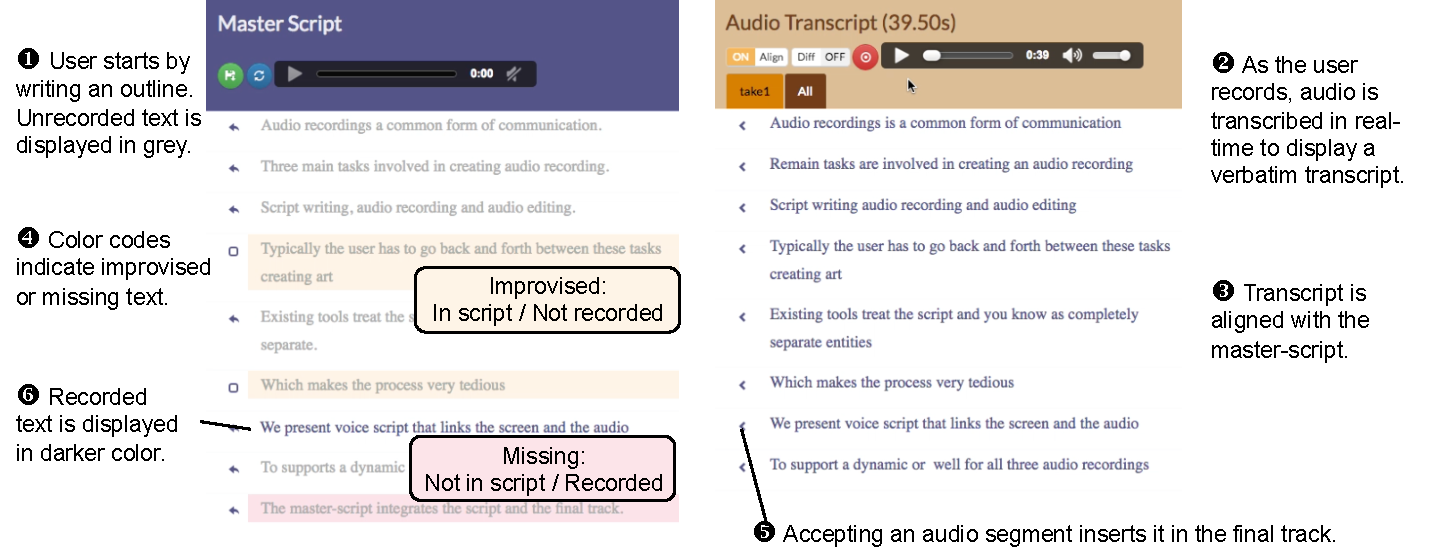
\includegraphics[width=2.0\columnwidth]{figures/ui_aligned}
  \caption{The \systemname\ interface. The master-script (left)  reflects the current state of
the project, including unrecorded script and recorded final track. As the user records, speech is transcribed in real
time and a verbatim text corresponding to each take appears in
a separate transcript document (right).}~\label{fig:ui_aligned}
\end{figure*}

\textbf{Text-based representation of audio.} We build on previous work~\cite{casares2002simplifying,whittaker2004semantic,berthouzoz2012tools,rubin2013content} that demonstrates the benefits of text-based representations of spoken audio for navigation and editing. \systemname\ uses automatic speech recognition (ASR) to transcribe audio recordings in realtime and represent each take with a verbatim transcript. As with previous systems, edits to these text transcripts are automatically propagated to the audio, which facilitates simple audio editing tasks. 

\textbf{Master-script view.} To help users manage the relationship between scripted text and recorded speech, we introduce the notion of a \emph{master-script} that shows a unified view of both unrecorded portions of the script and recorded speech included in the final track. By representing and visualizing both recorded and unrecorded text, the master-script provides a complete, readable view of the current state of the project that evolves as the user records and adds new takes to the final track, edits recorded text, or adds/modifies text that must be recorded. 

\textbf{Merge process.} Since recorded text typically differs from the script, \systemname\ provides an interface for merging changes into the master-script. The fact that we represent all recorded audio as text allows us to use standard text differencing to identify conflicts and execute merges. One key difference between our scenario and standard text merging is that recorded audio cannot simply be cut and merged into the master-script at any arbitrary word boundary. In many cases, the temporal gap between spoken words is not big enough to produce a seamless edit in the final track. Our merge interface takes this into account and helps the user execute merges that are likely to be artifact-free.

% As shown in Figure~\ref{interface}, our interface consists of two types of documents: a \textit{Master Script} document (left) displays the current status of the final track, including what has been recorded and what was planned to be recorded but has not been recorded yet (i.e. the original script), while a \textit{Transcript} document (right) displays the verbatim transcript of individual audio takes. As the user records new takes, our tool aligns the audio transcripts to the master script so that it is easy to compare each take with the master script and with each other. It also partitions each recording into segments that can be seamlessly joined between takes. At any point during the recording process, the user can edit the script or the final track by editing the master script like a text document.

\subsection{Interface and Usage Scenario}
The rest of this section describes our interface using an example scenario of how a user might create an audio recording. 

Typically, the user begins by writing an outline of points to record in the master-script.
The text appears in light grey to indicate that these parts have not been recorded yet (Figure~\ref{fig:ui_aligned} \textit{left}). At this stage, the master-script is like an ordinary, editable text document. 

Once the user starts recording, the audio is transcribed in real time and verbatim text corresponding to each take appears in a separate transcript tab (Figure~\ref{fig:ui_aligned} \textit{right}). Each transcript is time-aligned with the corresponding recording, so the user can quickly navigate to specific
parts of the audio by clicking on a word in the transcript. 

The next task is to decide which parts of the recording to merge into the master-script. To this end, we provide a \textit{compare-view} that aligns segments of the recording transcript to corresponding segments in the master-script and shows them side-by-side. To indicate improvised portions of the audio, any segment of the transcript that does not correspond to any part of the master-script is highlighted in yellow. To indicate mission portions in the audio, any segment of the master-script that does correspond to any part of the transcript is highlighted in red. To
view more detailed discrepancies between the script and recording, the
user can enable a \textit{diff-view} that displays per-word differences
using standard track change markers (i.e., strikethroughs for
missing words and highlighting for added words). 

To add recorded audio to the final track, the user can \textit{accept} any portion of the recording by clicking a button next to the appropriate transcript segment. If there is a corresponding segment in the master-script, the accepted transcript segment replaces it. If there is no corresponding master-script segment, the accepted transcript segment is simply inserted into the master-script. Within the master-script, accepted segments appear in black to indicate that these are recorded portions of text that have been added to the final track. 

%\VTODO{Mention the ability to revert?}

If the user records multiple takes, in addition to each of the transcript tabs, the \textit{all} tab provides a summary of all of the takes. For each segment in the master script, this tab displays all the corresponding transcript segments from all of the audio takes. A drop-down button next to a transcript segment  indicates that there are multiple versions (or takes)  of the  segment. Clicking on the button opens a list showing the alternative versions (Figure ~\ref{fig:multipletakes}). The user can listen to any of these takes and select one without having to search through individual takes. 
When the \textit{all} tab is in focus, any part of the master-script that has not been recorded in any of the takes is highlighted in red. In this way, the user can tell at a glance what has already been recorded and what still needs to be recorded. All of the dark (i.e. recorded) text in the master-script represents the current state of the final audio track; all of the grey text has not been recorded or is recorded but the author has not yet accepted it into the final track. 

During any point in the process, the user can edit the master-script
like a text document.  For example, the user can simply insert
more text to record or make changes to unrecorded text to flesh
out the original outline. \VREV{These edits can include verbatim script as well as comments or stage directions (e.g., "include examples" or "speaker softer" etc.).
The user can also edit or delete recorded portions of the text. Deleting recorded text from the master-script will remove the corresponding portion of the audio from the final track. Altering recorded text can introduce audio artifacts (e.g., when a word is deleted mid-sentence), or it could mean that the corresponding text no longer match the underlying audio. These parts are italicized and marked blue to remind the user to review or re-record relevant portions. Finally, the user has an option to correct the transcription of recorded words without affecting the underlying audio} \VTODO{(Figure~\ref{fig:transcription_correction}).} 

\subsection{Iteration and Asynchronous Collaboration}
\VREV{In order to produce the final recording, the user  often iterates back
and forth between all of these operations, editing the master-script,
recording audio takes, comparing alternative takes and accepting
audio segments into the final track.
 It is also common for multiple people to collaborate on a single voice-over. For example, a narrator who records the voice-over may work with others who write/edit the script, or several people may work on a recording with multiple voices. \\ In both iterative and collaborative editing, users need to identify (1) new content that needs to be recorded for the first time, and (2) existing content that needs to be re-recorded after the script edits. To visualize this information,  \textit{Voice Script} keeps track of per-word metadata about whether a word is unrecorded (grey), recorded and unedited (black), or recorded and edited (blue italics). For collaboration, this metadata is passed between users with the script and recordings. The visualization and the text-based  editing/merging interface facilitates audio editing even when different persons work on different parts of editing the script, recording the audio and/or re-arranging the recorded audio.   
}

\begin{figure}
\centering
  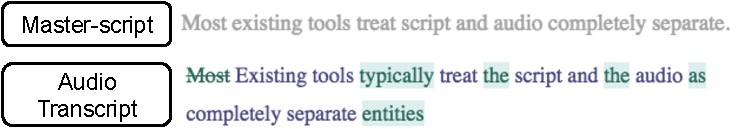
\includegraphics[width=1.0\columnwidth]{figures/diffview}
  \caption{The \textit{diff-view} displays a per-word difference between the master-script and the audio transcript.}~\label{fig:diffview}
\end{figure}

% \VTODO{Instead of describing all the different text colors throughout the section, it might be a bit clearer to skip all descriptions of text colors above and add a paragraph here saying that we visualize the text in the master-script with different colors to help users understand the state of the document. Red mean unrecorded, dark is accepted, etc.}


One key benefit of our interface is that it supports a wide range of workflows for different users and scenarios. For instance, instead of starting with a written outline, the user can begin with an empty master-script, start recording, and then use  the initial recording as an outline. The user can also record the entire script in a single take, or work on a single section at a time. 
\VREV{To create the voice-over for the supplementary video to this paper, two of the paper authors collaborated on \textit{Voice Script}. We also look at various workflows in our informal user evaluation.}

\section{Algorithmic Methods}
\label{sec:algorithms}
\subsection{Transcribing the audio recording}
We use IBM Speech to Text Service \cite{ibmspeechtotext} to obtain a verbatim transcript of each audio take in real time. The service produces a time stamp for each word indicating its start and end time. It also segments the transcript into \textit{utterances} where each utterance is separated by a longer silent gap in the speech (longer than 500 ms). While automatic speech recognition is imperfect, we have found that the results were accurate enough for the purpose of alignment (next section) and for understanding the transcript.
  
\subsection{Co-segmenting and aligning the transcript to the master script}
Once we have a verbatim transcript of an audio take, we compute the global word-to-word alignment between the transcript and the master script using the Needleman-Wunsch (NW) algorithm \cite{needleman1970general}. NW allows for insertions and deletions, which accounts for differences in the two documents for example, due to loose scripts, or inaccurate reading or transcription.

In order to display corresponding parts in the master script and the transcript side-by-side, we need to also segment the the two texts. Ideally, these segments will satisfy several conditions:  (1) In the case of typed, unrecorded text, these correspond to punctuations such as periods, commas or line breaks, whereas in recorded text, these correspond to longer pauses in the speech. 


\subsection{All tab view ?}
\subsection{Text edit markup ?}

\section{Results}
\VTODO{Voiceover for the we made and collaborative user scneario}

\section{Informal User Evaluation}
To gauge the utility of our interface, we conducted an informal evaluation with two users. We started each session with a brief demonstration of our interface, and then asked the participants to create an audio recording. We examined their workflow, and the number/type of features they used. We also solicited written qualitative feedback about our interface at the end of the session. Each session lasted about 50 minutes.


We also conducted a pilot study to compare our interface with a state-of-the-art transcript-based speech editing interface \cite{rubin2013content}. We recruited four participants, none of whom had experience using text-based audio editing systems. We gave them a script with bullet points outlining a mini lecture on a science subject (e.g. \textit{gravity} and \textit{dark matter}) and two audio takes roughly corresponding to that script. Their task was to cut and merge the two takes to produce a recording that contained all the contents listed in the script and only those contents. The two takes were similar, but both takes had some
missing content from the outline and one had some extra
content. So, the participants had to choose parts from each take and combine them to get the final result. Each participant completed the task twice with different outlines, once using our interface and the other using Rubin et al.'s interface. The subject of the outline and the order of the interface was counter-balanced. After the session, participants gave written qualitative feedback about the two interfaces. In total, each session lasted one hour.   
 

\section{Comparative study}
We also conducted a pilot study to compare our interface with
a state-of-the-art transcript-based speech editing interface
\cite{rubin2013content}. We recruited four participants, none of whom had
experience using text-based audio editing systems. We gave them
a script with bullet points outlining a mini lecture on a science
subject (e.g. \textit{gravity} and \textit{dark matter}) and
two audio takes roughly corresponding to that script. Their task
was to cut and merge the two takes to produce a recording that
contained all the contents listed in the script and only those
contents. The two takes were similar, but both takes had some
missing content from the outline and one had some extra
content. The participants had to choose parts from each take
and combine them to get the final result. We encouraged the users
to focus on having the complete content rather than the details
of the audio quality (e.g. tempo, diction, flow of speech etc.).

In Rubin et al.'s system (referred to as
\textit{Interface-R} hereafter), as in our interface, users
can edit the transcript like a text document using operations
such as copy-and-paste, insert or delete, and the edits are propagated
to the audio. The system  also detects alternate takes of the
same sentence and groups them for users to select between them.
However, unlike \systemname , Interface-R is geared for editing pre-recorded
audio, and does not support scripting or real-time recording.
In fact, it only allows editing one recording at a time. To simulate multiple takes, we took advantage of their multi-column interface, so that each take appeared in a separate column one after the other as if they were spoken by two different speakers. In \systemname,  the script was contained in the master-script, whereas in Interface-R, we gave users a hardcopy of the script.

Each participant completed the task twice with different outlines,
once using our interface and the other using Interface-R.
The subject of the outline and the order of the interface was
counter-balanced. We examined the time they spent editing,
the number/type of functions they used, and the quality of the
final recording (Table~\ref{}). After the session, participants gave written
qualitative feedback about the two interfaces. In total, each
session lasted 1 hour.
   
Each of the four participants preferred \systemname\ over Interface-R for the given task, and noted they would use
our interface to edit audio recordings. Every participant also
completed the task faster using our interface (7.4 $vs$ 9.9 min Interface-R). 

\VTODO{Explain usage}

All of the participants commented on how the master-script helped them in the task. One person noted that in \systemname\ \textit{``the master-script linked the two takes into one comprehensive view
that made the editing a lot simpler, [while in Interface-R] I felt like I had to consider two separate documents and combine them manually.''} Another person preferred the \systemname\ interface for the task of editing the audio content, and commented that Interface-R would be useful to make detailed edits to the speech flow. 3 out of the 4 participants also found the color-coded visualization of the master-script (recorded vs. unrecorded) and the transcript (planned vs. improvised) very helpful. A participant wrote about the \textit{compare-view} feature that \textit{``The alignment was great. I felt like almost half of my work was
already completed before I began.''} 



\section{Limitations}
\VREV{We rely on automatic speech recognition (ASR) to transcribe the audio recordings in real time. Despite recent improvements in ASR} \cite{hinton2012deep}, \VREV{its performance varies widely. Transcription errors can affect the user's performance negatively (e.g., in navigating the audio, or if the user has to spend time correcting the errors)} \cite{gaur2015effects}. \VREV{Currently, in \textit{Voice Script}, users can click on a word to listen to its corresponding audio and manually correct the transcription without affecting the audio. Better ways to fix or reduce ASR errors, for instance, taking advantage of the written script, is an interesting area for future work.} 

\VREV{We have used \textit{Voice Script} to collaborate \textit{asynchronously} to create voice recordings. Additional features are required in order to support synchronous collaboration. For instance, some type of conflict resolution and version control to keep track of the development would be useful.}

\VREV{Also, our interface focuses on the content of the speech recordings but does not consider editing details for audio quality. As one user mentioned in the feedback, we could integrate editing tools such as the ones in Rubin et al. }\cite{rubin2013content} or \cite{rubin2015capture} \VREV{to fine-ßtune audio quality. Speech recordings often accompany visual footage or other sound effects such as music that is also closely related to the script/audio. Future work could investigate how to integrate these contents in the workflow.}

\section{Conclusion and future work}
To create speech recordings, people iterate back and forth between script writing/editing and audio recording/editing.  \VREV{It is also common for several people to collaborate in the authoring workflow.} Unfortunately, most existing tools treat the script and the audio as completely separate entities, which makes the dynamic workflow between them very tedious. We presented \systemname, an authoring interface that facilitates integrated workflows for script writing and  audio recording/editing. \systemname\ introduces the notion of a \emph{master-script} that combines the script with the audio and unifies the script/audio editing task. Our system supports a wide range of workflows, \VREV{including asynchronous collaboration}, and facilitates novice users creating speech recordings. 






\section{Acknowledgments}


% BALANCE COLUMNS
\balance{}

% REFERENCES FORMAT
% References must be the same font size as other body text.
\bibliographystyle{SIGCHI-Reference-Format}
\bibliography{paper}

\end{document}

%%% Local Variables:
%%% mode: latex
%%% TeX-master: t
%%% End:
